\documentclass{article}

\usepackage{graphicx}
\usepackage{hyperref}
\usepackage{placeins}
\usepackage{subcaption}

\begin{document}

Machine Learning 2, exercise 3 by Constantin Pape, Marcus Theisen and Johann Klaehn
 
\section{Exercise and data}

In this exercise we implemente different neural networks and test them on the MNIST - dataset.

\section{Networks}

We use 2 fundemantelly different types of networks:
A two hidden layer network and a convolutional network.
The two layer network is used in three different configurations:
\newline 
In the standard configuration, with rectifiying activation function, with dropout, with dropout and PreLu activation.
\newline
Dropout works by randomly droping neurons from the network in each training iteration, thereby
reducing the overfitting, by preventing the weights learning patterns specific to the training data. However in the prediction the full network is used. That is why we need to initialise two models, one with dropout activated, one without.
\newline
In all these cases the network architecure stays the same:
625 hidden units in the first layer, 625 in the second layer and 10 (with softmax activation)
in the output layer.
\newline
For the convolutional network, we use 3 convolutional layers, each with a filter and subsampling layer. The last of these layers is connected to the second hidden layer (from before). The exact configuration is depicted in \autoref{fig1}.

%\begin{figure}[h]
%	\centering
%	\includegraphics[width = .8\textwidth]{graphics/conv_net.png}
%	\caption{Architecure of the Convolutional Net.}
%	\label{fig1}
%\end{figure}

\section{Results}

We train each network with the RMSProp algorthm on a training subset for 100 iterations 
(feasible thanks to the GPU).
It is then evaluated on a test subset.
In \autoref{tab1} the result for each network is shown.
\autoref{fig2} shows the course of the test classification rate over the training iterations.

\begin{table}[h]
	\centering
	\begin{tabular}{l c c c C}
        Model	&	Simple	& Dropout & PreLU   & Convolutional	\\
        Result	&	0.9852	& 0.9868  & 0.9871  &	0.9943      \\
	\end{tabular}
	\caption{Test classification after training.}
	\label{tab1}
\end{table}

\begin{figure}[h]
	\centering
	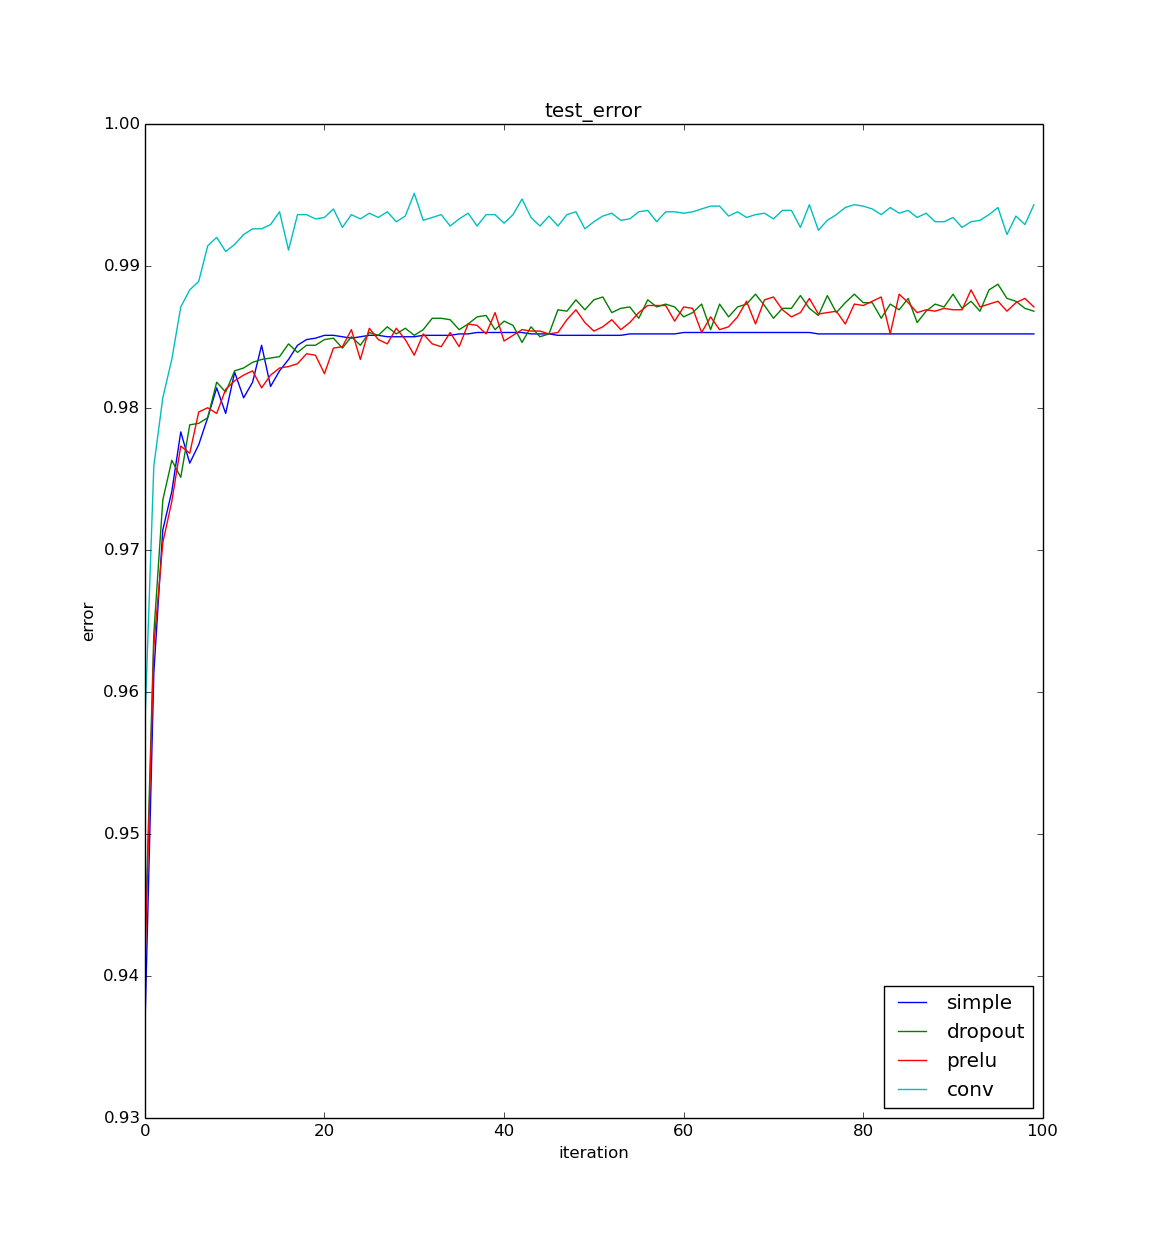
\includegraphics[width = .8\textwidth]{graphics/compare_nets.png}
	\caption{Test classification over iterations.}
	\label{fig2}
\end{figure}

As we can see the convolutional net outperforms the other networks w.r.t both, convergence rate and resulting classification rate. 
The 3 networks relying on the same architecure show very similar convergence, however Dropout and PreLU converge to a little better classification rate.
In contrast to the simple case, they show more noise, which is due to the fact that both of them use dropout during training.

\section{Filters}

To investigate the Convolutional Net further, we look at three filters from the first convolutional layer.
For this we convolve these filters with an image from the dataset and look at the convolution and the filter.
In \autoref{fig3} the image is shown.

\begin{figure}[h]
	\centering
	\includegraphics[width = .8\textwidth]{graphics/digt.png}
	\caption{Test classification over iterations.}
	\label{fig2}
\end{figure}



%\begin{figure}
%	\centering
%	\begin{subfigure}[b]{0.45\textwidth} 
%		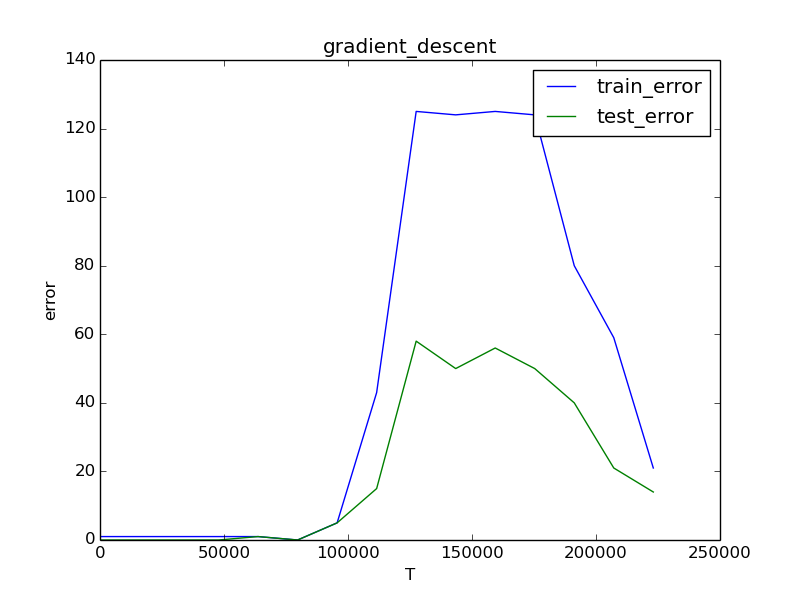
\includegraphics[width=\textwidth]{../results/gradient_descent.png}
%		\caption{Results for gradient descent}
%		\label{fig3}
%	\end{subfigure}
%	\begin{subfigure}[b]{0.45\textwidth} 
%		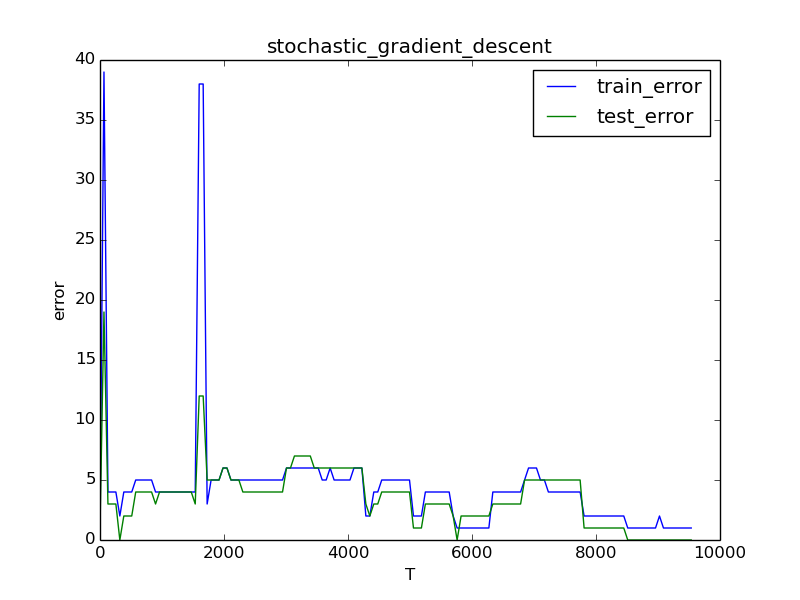
\includegraphics[width=\textwidth]{../results/stochastic_gradient_descent.png}
%		\caption{Results for stochastic gradient descent}
%		\label{fig4}
%	\end{subfigure}
%\end{figure}

\end{document}

